\section{Einleitung}

\ac{iot}

\subsection{Motivation}

\begin{displayquote}
  \glqq Wenn Technologien und Gesellschaft sich schneller ändern, als Unternehmen in der Lage sind sich anzupassen, dann kommt es ganz nach den Regeln der Evolution zum Austerben bestimmter Unternehmenstypen.\grqq{}
\end{displayquote}

\begin{flushright}
  \citet[S. 3, zitiert nach Land, K.-H. 2015]{Roth2016}
\end{flushright}

Wie das obige Zitat andeutet, erweist sich die Fähigkeit zur Adaption an neue Technologien durch Digitalisierung als Schlüssel für den Unternehmenserfolg. Diese Fähigkeit ermöglicht Unternehmen, durch die erlangene Schnelligkeit, Flexibilität und Produktivität ihre Effizienz zu steigern \citep{Roth2016}.
\\4. Industrielle Revolution und das ihr zugeschriebene Potenzial beschreiben. Viele Branchen profitieren aber es gibt eine Branche,
ohne die die Revolution zu einem nicht möglich wäre und die zum anderen auf sie angewiesen ist.
Die Energiebranche ist aufgrund der steigenden Nachfrage, durch immens zunehmende Vernetzung und Digitalisierung, mehr als je zuvor auf intelligente und effiziente Prozesse angewiesen.
Digitalisierung und Dezentralisierung in der Energiewirtschaft und so. In Energiewirtschaft wird außerdem \ac{sapisu} ausschließlich benutzt.
Es findet ein Sprung in das Zeitalter des \glqq Utility 4.0\grqq{} statt \citep{Doleski2017}.
Umstieg auf erneuere Energien durch Energiewende, Ausstieg aus Kernkraft mit 2022. Der Markt bringt intelligente Messsysteme für dezentrale Energieerzeugung wie die Smart Meter Technologie als Enabler für
die Digitalisierung auf den Markt. Dennoch gibt es viele alte Technologien.
Hier bisschen weitläufiger die Digitalisierung in Energiewirtschaft beschreiben mit Bezugnahme auf den Vertrieb,
die Verfügbarkeit, Erfüllen von Kundenwünschen, digitale Multi-Channeling Plattformen

Der Bedarf an Rechenleistung nimmt weiter zu
Viele Anwendungen von IKT sind in den vergangenen Jahren komplexer geworden und erfordern mehr Rechenleistung. Dieser Trend wird sich künftig im Zuge der weiteren Digitalisierung fortsetzen. Um mehr Rechenleistung bereitzustellen und den Anstieg des Energie- und Ressourcenbedarfs der Rechenzentren zu begrenzen, muss deren Effizienz erheblich steigen.

\begin{itemize}
  \item https://www.bdew.de/energie/digitalisierung/was-bedeutet-der-trend-der-digitalisierung-fuer-die-energiewirtschaft/
\end{itemize}

% Problemstellung
\subsection{Problemstellung} \label{problemstellung}
Monitoring der Sensorwerte einer Windenergieanlage mit SAP-Technologien mit geschlossenem Kreis -> Sensorwerte lösen Aktion wie SMS aus
\newline
Da in der Energiewirtschaft langfristige und teure Investitionsgüter bestehen, können Sie nicht einfach durch neue
digitalisierte Güter ersetzt werden. Umso mehr besteht die Herausforderung, alte Techniken mit neuen Technologien
auf die Digitalisierung vorzubereiten. Wir haben zum Beispiel eine alte Windenergieanlage, die nicht mit den
notwendigen Sensoren ausgestattet sind. Es soll trotzdem ermöglicht werden, Konditionen der Anlage und dessen Umgebung
zu überwachen, um z.B. Wartungsmaßnahmen auszulösen. -> Predictive Maintenance

\begin{itemize}
  \item Technologien zwar bereits im Einsatz aber sind gekapselt -> Insellösungen
  \item Mehrwert durch integrierte Nutzung mit Stammdaten (liegen im SAP System)
  \item SCADA z.B. bereits vorhanden aber Daten nicht intelligent vernetzt
\end{itemize}


\begin{itemize}
  \item[\textbf{FF1}] \textbf{Wie kann SAP Leonardo die digitale Transformation in der Energiewirtschaft mit Internet of Things unterstützen?}
  \begin{itemize}
    \item[FF1.1] Welche Anforderungen an ein System ergeben sich aus Sicht der dezentralen Ernergieerzeugung?
    \item[FF1.2] Welche Möglichkeiten zur intelligenten Vernetzung bietet die zugrundeliegende Systemarchitektur?
    \item[FF1.2] Mit welcher Systemarchitektur können die Anforderungen aus FF1.1 erfüllt werden?
  \end{itemize}
\end{itemize}

\subsection{Lösungsansatz}

Da Energiebranche ausschließlich mit \acf{sapisu} ihre Geschäftsprozesse verwaltet, liegt eine digitale Transformation
mit SAP-Produkten nahe. Dazu wurde ein Raspberry Pi 3 mit entsprechender Sensorik für die Simulation einer Windenergieanlage
ausgestattet. Die gemessenen Werte wurden an den Internet of Things Service der SAP Cloud Platform gesendet und anschlißend
einem digitalen Zwilling übergeben. Um den Zwilling mit entsprechenden Messwerten und Grenzüberschreitungen
sichtbar zu machen, wurde eine SAP UI5-Anwendung entwickelt. Um aus den gemessenen Werten einen Mehrwert zu gewinnen,
wurde ein \acf{aws} \acf{sns} angebunden, der bei Grenzüberschreitung bestimmter Messwerte eine
SMS-Benachrichtigung versendet. All diese Maßnahmen werden prototypisch implementiert

\begin{figure}[ht]
  \centering
  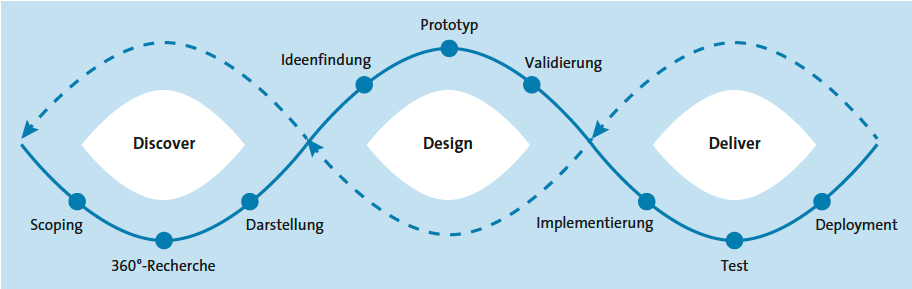
\includegraphics[width=\linewidth]{design_thinking}
  \caption[Phasen des Design-Thinking-Prozesses]{Phasen des Design-Thinking-Prozesses \citep[S. 69]{Elsner2018}}
  \label{}
\end{figure}

\subsection{Aufbau der Arbeit}



\begin{itemize}
  \item Zunächst Industrie 4.0 und treibende Faktoren allgemein
  \item Was ist der Mehrwert von Kommunikationssystemen und welche Protokolle sind Grundlage für die Vernetzung?
  \item Welche Referenzarchitektur vereinheitlicht industrielle Standards und Anforderungen an die Systeme?
  \item Was ist Cloud Computing und welche Rolle spielen dessen Technologien für Industrie 4.0?
  \item Welche Toolsets sind für die Lösung vorhanden?
  \item Use Case: Für welchen Anwendungsfall in der Energiebranche wird ein Prototyp entwickelt?
  \item Was sind die Anforderungen an den Prototypen? Näherer Bezug auf Energiebranche.
  \item Welche Komponenten besitzt das entworfene System bzw. sind notwendig?
  \item Wie sieht die Implementierung im Detail aus?
  \item Evaluierung des Vorgehens
  \item Fazit
\end{itemize}



\newpage
